\section{Front-end}

\frame{
    \frametitle{Front-end}
    \framesubtitle{Overview}
    \begin{enumerate}
    \item Error handling within the parser monad
    \item Order of the front-end
    \item Moving functionality from the type-checker to the parser
    \item Normalizing
    \item Type-checking
    \item Codegen interface
    \end{enumerate}
}
\subsection{Error handeling}

\frame{
    \frametitle{Error handeling within the parser monad}
    \begin{multicols*}{3}
    
    Concat all the errors
    \begin{enumerate}
    \item Slow
    \item Get all the errors and thus none
    \end{enumerate}

    \columnbreak

    Give only the last viable error
    \begin{enumerate}
    \item Fast
    \item posibility to lose error information
    \item posibility to get incorrect error information
    \end{enumerate}

    \columnbreak

    Priority for errorszz
    \begin{enumerate}
    \item Fast
    \item More accurate error information
    \item posibility to get incorrect error information
    \end{enumerate}
    \end{multicols*}
}

\frame{
    \frametitle{Errors with priority}
    \begin{figure}
        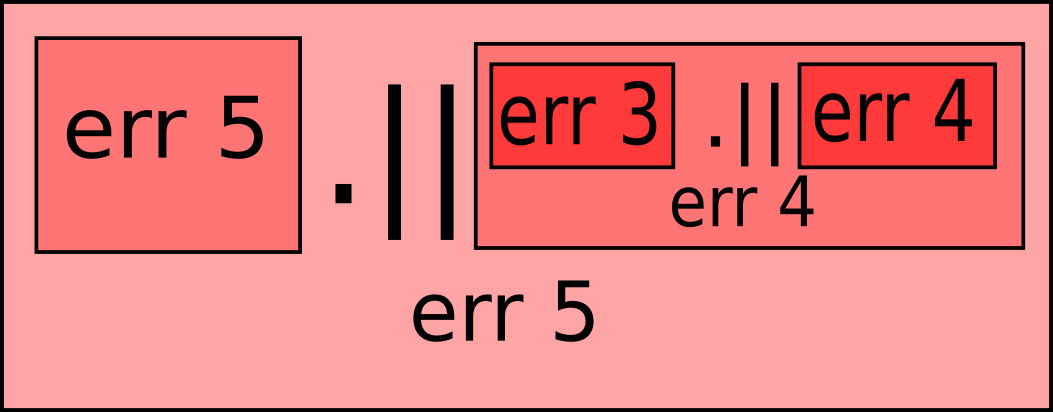
\includegraphics{error_example}
    \end{figure}
}


\subsection{Moving functionality from the type-checker to the parser}

\frame{
    \frametitle{Moving functionality from the type-checker to the parser}
    \begin{enumerate}
    \item Order of the front-end
    \item Identification of variable kind's
    \item Identification of function names
    \item Detection of partial application
    \item Building an expresiontree within a sentence
    \end{enumerate}

}

\frame{
    \frametitle{Order of the front-end}
    Parsing $\longrightarrow$ Type-checking $\longrightarrow$ Normalizing $\longrightarrow$ Back-end

    Parsing $\longrightarrow$ Normalizing $\longrightarrow$ Type-checking  $\longrightarrow$ Back-end
}

\frame{
    \frametitle{Identification of variable kind's}
    Incorporating kind information in the syntax.
    
    \begin{itemize}
    \item Incorporating kind information in the syntax.
    \item Type has an apostrophe before its variable name. Example (‘a ,’generic, ‘type-variable)
    
    \item Kind has a sharp before its variable name. Example (\#kind, \#module, \#term, \#type)
    \end{itemize}
}

\begin{frame}[fragile]
    \frametitle{Identification of function names}
    
    \begin{lstlisting}
    Func 'a -> "add" -> b' -> Tuple <'a 'b>
    \end{lstlisting}

    \begin{lstlisting}
    Prs{
        let! larg = parse_left_arg
        let! name = check_string “add”
        let! rarg = parse_right_arg
        let! res = parse_result
    }
    \end{lstlisting}

    Because all function have a declaration we can generate parsers specifically made to parse this one function definition. 

\end{frame}

\begin{frame}[fragile]
    \frametitle{Detection of partial application}   
    
    \begin{lstlisting}
    Func "add" -> int -> int -> int
    Func "foo" -> int -> int -> int
    add -> a0
    a0 x -> a1
    a1 y -> res
    -------
    foo x y -> res
    \end{lstlisting}
    \begin{lstlisting}
    a0 = int -> int -> int
    a1 = int -> int
    res = int
    \end{lstlisting}


\end{frame}